\pdfminorversion=7
\documentclass[12pt,twoside]{report}
\usepackage{srcltx}
\usepackage{epsfig}
\usepackage{graphicx,amssymb,amsmath,amsthm}
\usepackage{graphicx,color,enumerate}
\usepackage[rflt]{floatflt}
\usepackage{rotating}
\usepackage{caption2}
\usepackage{cases}
\usepackage{mathrsfs}
\usepackage{amsfonts}
\usepackage{multicol}
\usepackage{pstricks}


\topmargin 20mm      % the top margin is not less than 2 cm
\textheight 24.0cm
\textwidth 150mm
\oddsidemargin 35mm    % the binding margin is not less than 3.5 cm
\evensidemargin 25mm
%\evensidemargin 35mm

\headsep 0in
\voffset -28mm
\hoffset -25.4mm

\renewcommand{\contentsname}{\leftline{Table of Contents}}
\renewcommand{\theequation}{\thesection.\arabic{equation}}
\pagenumbering{roman}
\renewcommand{\baselinestretch}{1.6}\normalsize
\def\title#1{\def\ntitle{#1}}
\def\author#1{\def\nauthor{#1}}
\def\supervisor#1{\def\nsupervisor{#1}}
\def\degree#1{\def\ndegree{#1}}
\def\date#1{\def\ndate{#1}}
\newcommand{\Thesistitle}
{
\newpage
\null\vspace*{0.5in}
\begin{center}
	{\Large\bf \ntitle}

	\vspace*{3.5cm} {\large\bf \nauthor} \vspace*{2cm}

	{\bf A thesis submitted in partial fulfilment of the requirements

	for the degree of}

	{\normalsize \ndegree}

	\vspace*{3.5cm}


	{\normalsize\bf Principal Supervisor:}

	{\bf \nsupervisor \space (Hong Kong Baptist University)}

	\vspace*{2cm}
	{\normalsize \ndate}

	\thispagestyle{empty}
\end{center}
}


\newcommand{\thesis}
{
\newpage
\pagenumbering{arabic} \setcounter{chapter}{0}
\setcounter{section}{0} \setcounter{page}{1} 
}

\makeatletter
\renewcommand*\l@chapter[2]{%
\ifnum \c@tocdepth >\m@ne
\addpenalty{-\@highpenalty}%
\vskip 1.0em \@plus\p@
\setlength\@tempdima{1.5em}%
\begingroup
\parindent \z@  \rightskip \@pnumwidth
\parfillskip -\@pnumwidth
\leavevmode %\bfseries
\advance \leftskip 2.4cm %\leftskip\@tempdima
\hskip -\leftskip
#1\nobreak\hfil \nobreak\hb@xt@\@pnumwidth{\hss #2}\par
\penalty\@highpenalty
    \endgroup
    \fi}
    \def\@chapter[#1]#2{
    \ifnum \c@secnumdepth >\m@ne
    \refstepcounter{chapter}%
    \typeout{\@chapapp\space\thechapter.}%
    \addcontentsline{toc}{chapter}%
    {\bf \protect \numberline {Chapter \thechapter}\hspace*{1.5cm} {#1}}%
    \else
    \addcontentsline{toc}{chapter}{#1}%
    \fi
    \chaptermark{#1}%
    \addtocontents{lof}{\protect\addvspace{10\p@}}%
    \addtocontents{lot}{\protect\addvspace{10\p@}}%
    \if@twocolumn
    \@topnewpage[\@makechapterhead{#2}]%
    \else
    \@makechapterhead{#2}%
    \@afterheading
    \fi
    \renewcommand{\chaptermark}[1]{\markright{\chaptername \ \thechapter.\ #1}{}}
    }



    \makeatother



    \newtheorem{theorem}{Theorem}[section]
    \newtheorem{lemma}[theorem]{Lemma}
    \newtheorem{corollary}[theorem]{Corollary}
    \newtheorem{definition}[theorem]{Definition}
    \newtheorem{proposition}[theorem]{Proposition}
    \newtheorem{claim}{Claim}
    \newtheorem{conjecture}[theorem]{Conjecture}
    \newtheorem{model}{{ \bf Model}}[section]
    \newtheorem{assumption}{{ \bf Assumption}}[section]
    \newtheorem{remark}{{ \bf Remark}}

    \newtheorem{prop}{Proposition}
    \newtheorem{theo}{Theorem}


    \renewcommand{\captionfont}{\footnotesize \tt}
    \renewcommand{\captionlabelfont}{\footnotesize}

    \makeatletter
    \renewcommand*\l@chapter[2]{%
    \ifnum \c@tocdepth >\m@ne
    \addpenalty{-\@highpenalty}%
    \vskip 1.0em \@plus\p@
    \setlength\@tempdima{1.5em}%
    \begingroup
    \parindent \z@  \rightskip \@pnumwidth
    \parfillskip -\@pnumwidth
    \leavevmode \bfseries
    \advance \leftskip 2.5cm %\leftskip\@tempdima
    \hskip -\leftskip
    #1\nobreak\hfil \nobreak\hb@xt@\@pnumwidth{\hss #2}\par
    \penalty\@highpenalty
								    \endgroup
								    \fi}
								    \def\@chapter[#1]#2{\ifnum \c@secnumdepth >\m@ne
								    \refstepcounter{chapter}%
								    \typeout{\@chapapp\space\thechapter.}%
								    \addcontentsline{toc}{chapter}%
								    {\protect\numberline{Chapter \thechapter \ } \hspace*{1.5cm} #1}%
								    \else
								    \addcontentsline{toc}{chapter}{#1}%
								    \fi
								    \chaptermark{#1}%
								    \addtocontents{lof}{\protect\addvspace{10\p@}}%
								    \addtocontents{lot}{\protect\addvspace{10\p@}}%
								    \if@twocolumn
								    \@topnewpage[\@makechapterhead{#2}]%
								    \else
								    \@makechapterhead{#2}%
								    \@afterheading
								    \fi}
								    \makeatother

\usepackage{hyperref}
\usepackage{multirow}
\usepackage{algorithm}
\usepackage{algorithmic}
\usepackage[nottoc]{tocbibind}
\usepackage{seqsplit}

% it modifies all chapter titles at once
\usepackage{titlesec}
\titleformat{\chapter}[display]{\normalfont\bfseries\filcenter}{\huge\chaptertitlename\ \thechapter}{1ex}{\Huge}

% For quotes
\usepackage[english]{babel}
\usepackage[autostyle, english = american]{csquotes}
\usepackage{float}
\MakeOuterQuote{"}
% remove the box for each link and set the color
\usepackage{xcolor}

\usepackage[protrusion=true,expansion=true]{microtype}

\hypersetup{
    colorlinks,
    linkcolor={red!50!black},
    citecolor={blue!50!black},
    urlcolor={blue!80!black}
}
 % add a “List of Abbreviations”
\usepackage[acronym,nonumberlist,toc]{glossaries}
\makeglossaries

% Algorithm environment
\newcommand{\hash}[1]{{\ttfamily\seqsplit{#1}}}
\usepackage{abstract}
\renewcommand{\abstractname}{}    % clear the title
\renewcommand{\absnamepos}{empty} % originally center
\renewcommand{\algorithmicrequire}{\textbf{Input:}}
\renewcommand{\algorithmicensure}{\textbf{Output:}}

% For tables
\usepackage{booktabs} % For professional-looking lines (\toprule, \midrule, \bottomrule)
\usepackage{amsmath}  % For \text in math mode
\usepackage{array}    % For fixed-width columns
\usepackage{pdflscape}% For the landscape environment
\usepackage{rotating} % For rotated table headers (\sideways)
\usepackage{longtable} % For tables that span multiple pages
\usepackage{threeparttable}% For table-specific footnotes

\newcommand{\frontchapter}[2][]{%
  \cleardoublepage
  \phantomsection
  \chapter*{#2}%
  \if\relax\detokenize{#1}\relax
    \addcontentsline{toc}{chapter}{#2}%
  \else
    \addcontentsline{toc}{chapter}{#1}%
  \fi
}


\author{LI Lei}
\supervisor{Prof. SURNAME Name}

\title{Natural Language Explanation for Recommendations and Beyond}
\degree{Doctor of Philosophy}
\date{August 2025}

\begin{document}
\pagestyle{plain}

\pagenumbering{roman}

\Thesistitle

\newpage
\setcounter{page}{1}

\frontchapter[DECLARATION]{DECLARATION}
I hereby declare that this thesis represents my own work which has been done after registration for the degree of PhD at Hong Kong Baptist University, and has not been previously included in a thesis or dissertation submitted to this or any other institution for a degree, diploma or other qualifications.

I have read the University's current research ethics guidelines, and accept responsibility for the conduct of the procedures in accordance with the University's Research Ethics Committee (REC). I have attempted to identify all the risks related to this research that may arise in conducting this research, obtained the relevant ethical and/or safety approval (where applicable), and acknowledged my obligations and the rights of the participants.

\vskip 1cm

\hfill Signature:$\underline{\hspace{4cm}}$

\hfill August 2025

\newacronym{rnn}{RNN}{recurrent neural network}

\newpage
\phantomsection
\addcontentsline{toc}{chapter}{ABSTRACT}
\chapter*{ABSTRACT}
Your abstract


\vspace{1cm}

\noindent {\bf Keywords:} Explainable Recommendation, Explainable Artificial Intelligence, Recommender Systems

\newpage
\phantomsection
\addcontentsline{toc}{chapter}{ACKNOWLEDGEMENTS}
\chapter*{ACKNOWLEDGEMENTS}
I would like to thank Dr. Guozhong Li for the nice suggestion of making this template as well as the procedure open-source.

Thanks for the following update:

- By Li Lei, May 2022

- By XIONG Xin, Aug 2025


\newpage % Use this part to insert the table of contents
\phantomsection
\addcontentsline{toc}{chapter}{Table of Contents}
\renewcommand*\contentsname{Table of Contents}
\tableofcontents

\newpage % Use this part to insert the list of table.
% \addcontentsline{toc}{chapter}{List of Tables}
\listoftables

\newpage % Use this part to insert the list of figure.
% \addcontentsline{toc}{chapter}{List of Figures}
\listoffigures

\newpage % Use this part to insert the list of algorithm.
\addcontentsline{toc}{chapter}{List of Algorithms}
\listofalgorithms
\addtocontents{loa}{\def\string\figurename{Algorithm}}

\printglossary[
  type=\acronymtype,
  title=List of Abbreviations,
  toctitle=List of Abbreviations
]

\thesis % This command is used to set the page number.
\newpage


\chapter{Introduction} \label{ch:intro}
A brief introduction to this chapter.

\section{Motivation}

Sample citations: pre-trained GPT-2\footnote{Codes available at \url{https://github.com/lileipisces/PEPLER}} \cite{22-PEPLER}, Transformer \cite{ACL21-PETER}, \gls*{rnn} \cite{CIKM20-NETE}

\section{Outline}

\section{Contributions}

\begin{figure}
	\centering
	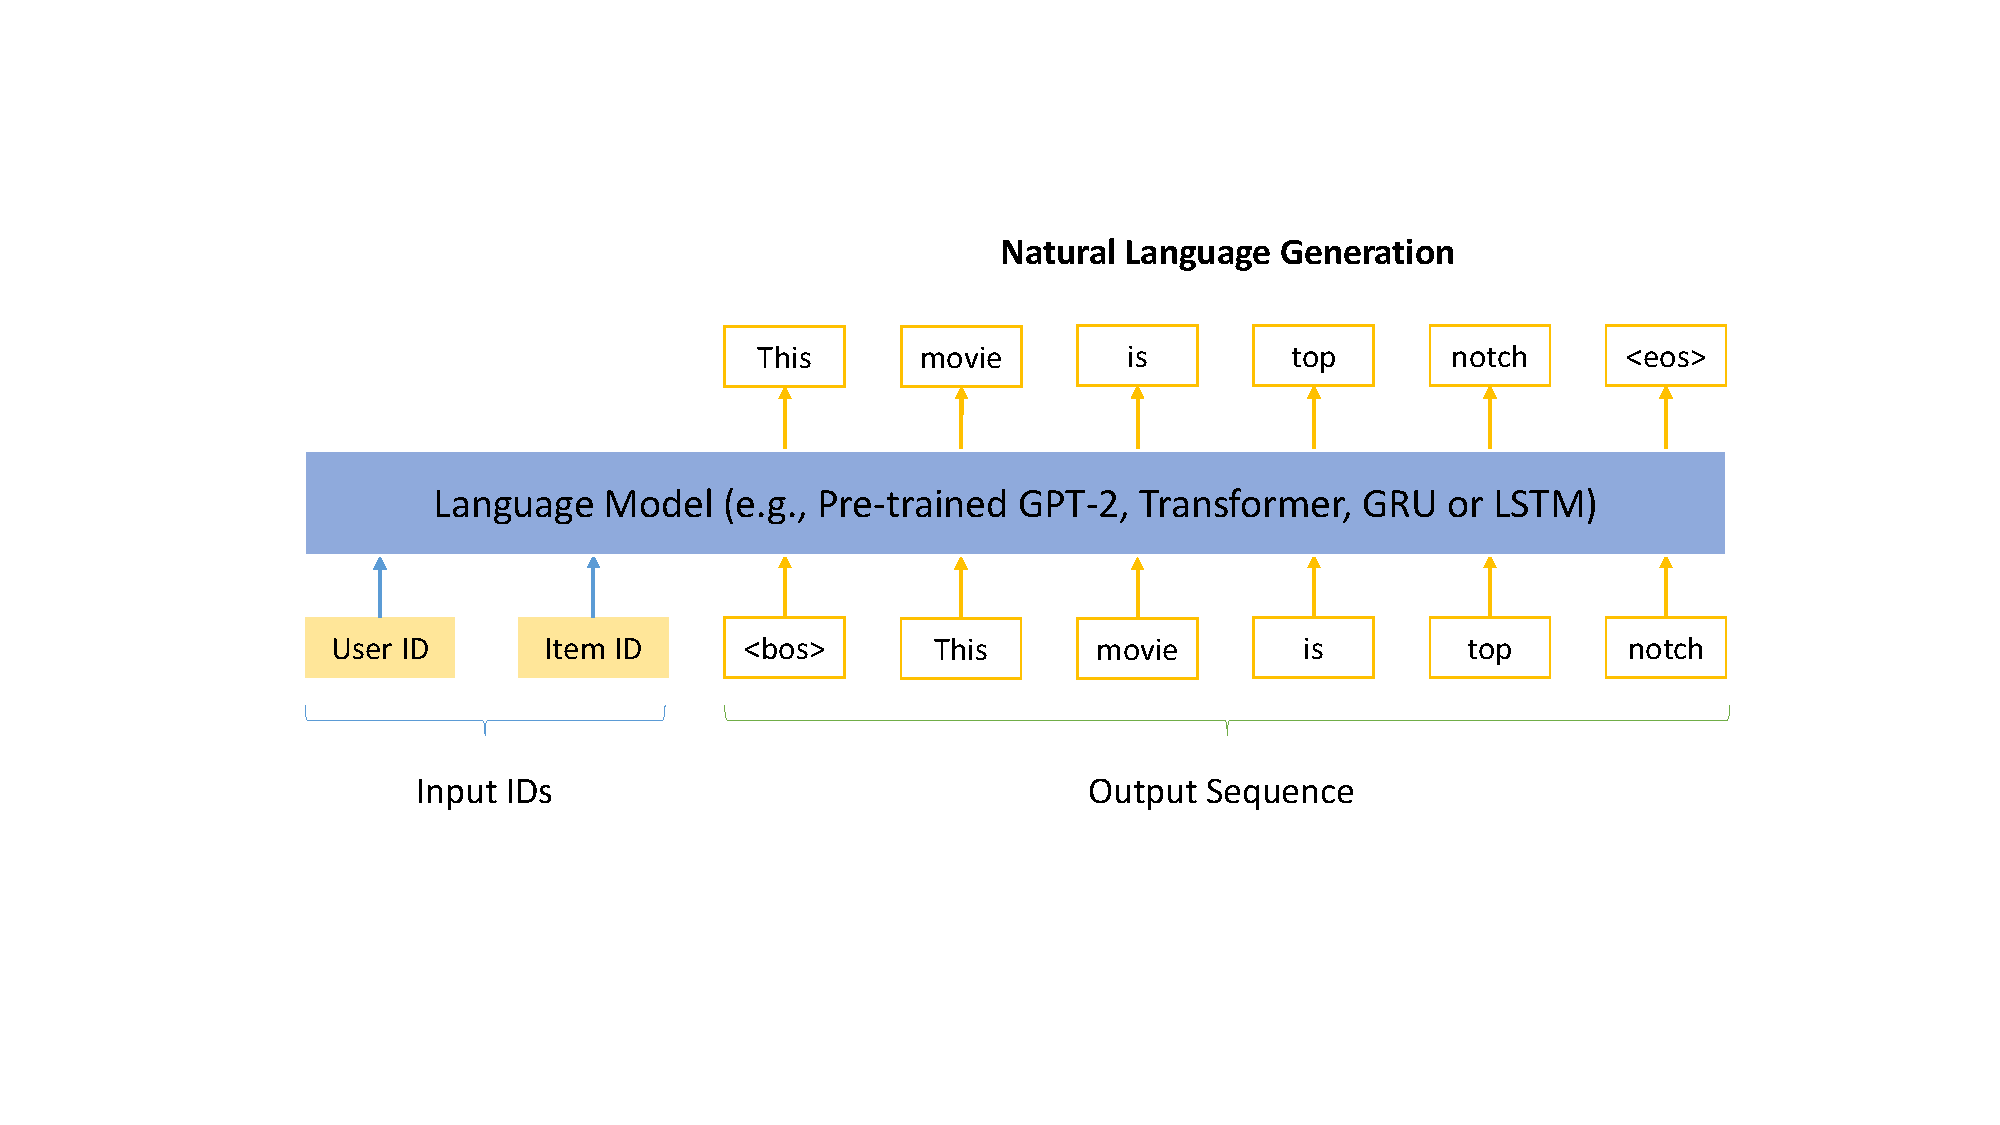
\includegraphics[scale=0.5]{fig/ch1/NLG4RS.pdf}
	\caption[Overview of recommender systems-based natural language generation.]{Overview of recommender systems-based natural language generation. In the case of recommendation explanation generation, the model is instructed to generate a word sequence for explaining why an item is recommended to the user.}
	\label{fig1:model}
\end{figure}

Use the following command to shorten the captions shown in List of Tables/Figures:
\begin{verbatim}
	\caption[shorter caption in List of
	Tables/Figures]{Real capation above or below the table/figure}
\end{verbatim}
See Fig. \ref{fig1:model} for example.


\chapter{Literature Survey} \label{ch:survey}


\section{Explainable Recommendation}


\section{Context-aware Recommendation}


\section{Natural Language Generation}


\section{Learning to Rank}



\chapter{Natural Language Explanation Generation} \label{ch:peter}
\section{Background}

\section{Problem Formulation} \label{sec3:problem}


\section{Model Description}


\subsection{Input Representation}

\begin{algorithm}
	\caption{Sentence Grouping via Locality-Sensitive Hashing (LSH)}
	\label{alg3:lsh}
	\begin{algorithmic}[1]
		\REQUIRE shingle size $n$, similarity threshold $t$, minimum group size $g$
		\ENSURE explanation set $\mathcal{E}$, groups of sentences $\mathcal{M}$
		\STATE Pre-process textual data to obtain the sentence collection $\mathcal{S}$
		\STATE $lsh \gets MinHashLSH(t)$, $\mathcal{C} \gets \varnothing$
		\FOR{sentence $s$ in $\mathcal{S}$}
		\STATE $m \gets MinHash()$  // create MinHash for $s$
		\FOR{$n$-shingle $h$ in $s$}
		\STATE $m.update(h)$  // convert $s$ into $m$ by encoding its $n$-shingles
		\ENDFOR
		\STATE $lsh.insert(m)$, $\mathcal{C}.add(m)$  // $\mathcal{C}$: set of all sentences' MinHash
		\ENDFOR
		\STATE $\mathcal{M} \gets \varnothing$, $\mathcal{Q} \gets \varnothing$  // $\mathcal{Q}$: set of queried sentences
		\FOR{$m$ in $\mathcal{C}$}
		\IF{$m$ not in $\mathcal{Q}$}
		\STATE $\mathcal{G} \gets lsh.query(m)$  // $\mathcal{G}$: ID set of duplicate sentences
		\IF{$\mathcal{G}.size > g$}
		\STATE $\mathcal{M}.add(\mathcal{G})$  // only keep groups with enough sentences
		\STATE $\mathcal{E}.add(\mathcal{G}.get())$  // keep one explanation in each group
		\ENDIF
		\FOR{$m'$ in $\mathcal{G}$}
		\STATE $lsh.remove(m')$, $\mathcal{Q}.add(m')$  // for efficiency
		\ENDFOR
		\ENDIF
		\ENDFOR
	\end{algorithmic}
\end{algorithm}

\subsection{Transformer and Attention Masking}



\subsection{Explanation and Recommendation}


\paragraph{Explanation Generation:}


\paragraph{Context Prediction:}


\paragraph{Rating Prediction:}


\paragraph{Multi-task Learning:}


\section{Experimental Setup}


\subsection{Datasets}

\begin{table}
	\caption{Statistics of the three datasets.}
	\begin{center}	
		\begin{tabular}{l|r|r|r}
			\hline
			& Yelp & Amazon & TripAdvisor \\
			\hline
			\#users & 27,147 & 7,506 & 9,765 \\
			\#items & 20,266 & 7,360 & 6,280 \\
			\#records & 1,293,247 & 441,783 & 320,023 \\
			\#features & 7,340 & 5,399 & 5,069 \\
			\#records / user & 47.64 &58.86&32.77 \\
			\#records / item & 63.81 &60.02&50.96 \\
			\#words / explanation & 12.32 &14.14&13.01 \\
			\hline
		\end{tabular}
	\end{center}	
	\label{table3:dataset}
\end{table}

\subsection{Evaluation Metrics}


\subsection{Compared Methods}


\subsection{Implementation Details}





\section{Results and Analysis}

\subsection{Quantitative Analysis on Explanations}


\subsection{Qualitative Case Study on Explanations}


\subsection{Recommendation Performance}


\subsection{Ablation Study}

\begin{sidewaystable}[!tbp]
	\caption[Ablation study on the smallest dataset TripAdvisor.]{Ablation study on the smallest dataset TripAdvisor. Arrows $\uparrow$ and $\downarrow$ respectively denote the performance increase and decrease compared with PETER.}
	\begin{center}
		\begin{tabular}{l|lll|lll|ll}
			\hline
			\multirow{2}{*}{} & \multicolumn{3}{c|}{Explainability} & \multicolumn{3}{c|}{Text Quality}  & \multicolumn{2}{c}{Recommendation} \\ \cline{2-9}
			& FMR & FCR & DIV & USR & BLEU-1 & BLEU-4 & RMSE & MAE \\ \hline		
			Disable $\mathcal{L}_c$ & 0.06 $\downarrow$ & 0.03 $\downarrow$ & 5.75 $\downarrow$ & 0.01 $\downarrow$ & 15.37 $\downarrow$ & 0.86 $\downarrow$ & 0.80 $\uparrow$ & 0.61 $\uparrow$ \\
			Disable $\mathcal{L}_r$ & 0.07 & 0.14 $\uparrow$ & 2.90 $\uparrow$ & 0.10 $\uparrow$ & 16.16 $\uparrow$ & 1.15 $\uparrow$ & 3.23 $\downarrow$ & 3.10 $\downarrow$ \\
			Left-to-Right Masking & 0.07 & 0.15 $\uparrow$ & 2.68 $\uparrow$ & 0.12 $\uparrow$ & 15.73 $\downarrow$ & 1.11 & 0.87 $\downarrow$ & 0.68 $\downarrow$ \\ \hline
			PETER & 0.07 & 0.13 & 2.95 & 0.08 & 15.96 & 1.11 & 0.81 & 0.63 \\ \hline
		\end{tabular}
	\end{center}
	\label{table3:ablation}
\end{sidewaystable}

\section{Summary}


\chapter{Conclusion and Future Work} \label{ch:conclude}


\section{Conclusion}

\section{Future Work}


\newpage
% \addcontentsline{toc}{chapter}{Bibliography}
\printbibliography[heading=bibintoc, title={Bibliography}]
% \bibliographystyle{plain}
% \bibliography{bibliography}

\newpage
\phantomsection
\addcontentsline{toc}{chapter}{List of Publications}
\chapter*{\centerline{ List of Publications}}

\begin{enumerate}
	\item {\sc \underline{Lei Li}, Yongfeng Zhang, Li Chen}, {\it Personalized Prompt Learning for Explainable Recommendation}, {\bf ACM Transactions on Information Systems}, 2022. [\textit{submitted}]
	\item {\sc \underline{Lei Li}, Yongfeng Zhang, Li Chen}, {\it Personalized Transformer for Explainable Recommendation}, {\bf Proceedings of the 59th Annual Meeting of the Association for Computational Linguistics and the 11th International Joint Conference on Natural Language Processing}, pages 4947-4957, Online, Thailand, August 1--6, 2021. ({\bf oral paper})
	\item {\sc \underline{Lei Li}, Li Chen, Ruihai Dong}, {\it CAESAR: Context-Aware Explanation based on Supervised Attention for Service Recommendations}, {\bf Journal of Intelligent Information Systems}, volume 57 (1), pages 147-170, August 2021.
\end{enumerate}


\newpage
\phantomsection
\addcontentsline{toc}{chapter}{CURRICULUM VITAE}
\chapter*{\centerline{ CURRICULUM VITAE}}

\noindent Academic qualifications of the thesis author, Mr. LI Lei:

$\bullet$ \ Received the degree of Bachelor of Engineering from Shenzhen University, June 2017. \\
\indent $\bullet$ \ Received the degree of Bachelor of Science from Shenzhen University, June 2017. \\
\indent $\bullet$ \ Received the degree of Master of XX from XX University, MM YYYY. \\
\vspace{1cm}

\hfill May 2022

\end{document}
